\documentclass[12pt]{article}

\usepackage[margin=1in]{geometry}
\usepackage[utf8]{inputenc}
\usepackage[british]{babel}
\usepackage{csquotes}
\usepackage{listings}
\usepackage[style=ieee,citestyle=numeric]{biblatex}
\usepackage{parskip}
\usepackage{graphicx}

\addbibresource{research.bib}
\setlength{\parskip}{1em}
\graphicspath{ {images/} }

\title{Exploring real time data collection and parameter monitoring in an Internet of Things system}
\author{Author: Henry David Rubiano Poveda \and Supervisor: Prof. Thomas Thomson}
\date{\today}

\begin{document}

\maketitle
\newpage

\begin{abstract}
    The Internet of Things has grown at an exponential rate over the past few years. The technological progress in the field has allowed us to integrate even further the Internet into almost every single area of society. Thanks to IoT we can now connect ``things'' to the Internet by embedding small devices, which can collect data, communicate between each other or even make decisions without almost any kind of human intervention. This IoT project explores data collection and monitoring by further developing and implementing a system able to collect data from a variety of sensors and send it to a database to store it over time. The project will go through different stages in which different areas will be explored and different solutions will be developed. First, the project will explore the range of hardware components to be used, along with the different software and database system. Then, it will emphasise on the importance of storage optimisation on devices with limited resources, following with the implementation of an intelligence system able to monitor the data and make decisions accordingly, in order to preserve the well-being of the system. The project will finish with the implementation of different logging systems to add an extra layer of reliability in terms of information storage. 

\end{abstract}
\newpage

\renewcommand{\abstractname}{Acknowledgements}
\begin{abstract}
    \setlength{\parskip}{1em}

    First, I would like to thank my supervisor Professor Thomas Thomson. His valuable help and support have been very important for me, and it was with his orientation and assistance that I was able to successfully develop this project. \par

    I would also like to thank my family and friends, who have helped me during these last 3 years and keep supporting me along the way. Thanks to them I have been able to get to this point, and I am forever grateful for their support.

\end{abstract}
\newpage

\tableofcontents
\newpage

\section{Introduction}

The Internet of Things is rapidly changing how we interact with the world around us, providing us with new more efficient ways of approaching real world problems by integrating technology in many more different areas of society. It is clear that in this new era, data is becoming a very valuable asset for many organisations, as it allows them to have more control over the decisions they choose to take. It also helps them keep track of many different vital system parameters over time, which will certainly be helpful, as they will be able to learn about their product using the experience that this data will provide them. This is why the collection of real time data is becoming more and more important as technology advances and becomes a crucial part of our daily life. \par 

It would certainly be complicated to encapsulate the Internet of Things into a single defined area or field, as we are starting to realise about the broad range of applications and possible different paths of development that can be explored within the topic. Now, the future will not consist of interaction between people, or even people interacting with the information and the data. The future will be about machines communicating with other machines in order to serve the people. Thanks to the Internet of Things, we are entering an era of total connectivity: Anywhere, anytime; where a new dimension has been added to this world of communication technologies \cite{future-internet}.\par

Along with the recent progress in the IoT field, the need for collecting data in different rooms or buildings has increased over the past few years. This is because better knowledge on the conditions of the building or its environment can help us greatly to gain a better understanding on the energy use, environmental quality, or many other different parameters that might be vital for some tasks. In order to achieve this, it is necessary to create a system that can monitor environmental parameters of the building or any specific room where this kind of system might be needed (rooms where experiments may be ocurring). These experiments need to be under control at all times, as changes as subtle as the increase of pressure may have a considerable effect on the outcome of the experiment. While many corporations provide this kind of service, they are usually limited by the use of proprietary hardware and software, which could also affect negatively costs, flexibility and scalability of the project, or even integration with the rest of the system. By using open source platforms and technologies, many opportunities for customisation and development of cost-effective systems with high levels of monitoring arise; and this helps the organisations to create their own solutions, and not depend on anybody but themselves \cite{building-science}.\par 

Monitoring data uninterruptedly requires storing large amounts of data. In order to achieve that, database systems with high levels of flexibilty and scalability are necessary, therefore emphasis should be placed on database schemas. While relational databases can deal with extremely large quantities of information, achieving efficient system scalability is considerably harder than the addition of new hardware components, therefore alternatives must be explored in order to develop this project in a more effective way \cite{nasar2019suitability}. 

\subsection{Aims and Objectives}

The main objective of this third year project is to explore the collection, pre-processing and transfer of real time data in an Internet of Things system, by further designing and implementing a system able to monitor parameters efficiently and effectively in a diverse range of instrumentation and equipment, while making decisions intelligently according to the different kinds of data collected from the environment. The project will try to expand on the previous project by assessing the current project version, create possible development paths for new functionalities or improvements to the current version and evaluate results. In order for this project to be carried out successfully, scalability and flexibility should be considered to be very important factors, as the project must be able to be further developed in the future.

\subsection{Structure} 

The structure of the report will consist on the following sections, that will explore in more detail some of the key aspects of this project:

\begin{itemize}
    \item First, the different topics that are explored in this project will be introduced, and a brief overview of the main aims and objectives will be described.
    \item Then, the report will try to give a comprehensive definition and background on the history of the Internet of Things, apart from describing its main purpose. This will be very important in order to properly understand the main motivations of the project. In this section the different applications of this field and its system architecture will also be explained. 
    \item The second section will consist on the Design and Approach. This section will contain some of the principal requirements of the project, a simple explanation of the system architecture that will be used, the hardware components selection and some of the most important aspects of the project, such as the concept of storing the specific type of data we are working with (time series data), the visualisation platform that will be used, and a brief overview of the security threats and features of the project.
    \item We will follow the previous section with the Implementation, where we will look in more detail the techniques used to expand on the previous developed version, which will consist of the new features of data collection, memory optimisation, data monitoring and data logging.
    \item We will finish the report evaluating our results and reflecting on the project, and arriving to conclusions that will certainly be useful for future further developments and progress. 
\end{itemize}

\section{Background}
\subsection{The Internet of Things}

\subsubsection{Definition}

According to the Oxford Dictionary, the Internet of Things (IoT) is “the interconnection via the Internet of computing devices embedded in everyday objects, enabling them to send and receive data”.  We should not confuse the Internet of Things with smart technology though, as this technology only refers to any device that is able to connect to the Internet. While we need to be present in order for a smart device (such as a smartphone) to use the technology and hence connect to the Internet, an IoT device could be accessed and controlled from anywhere at anytime \cite{french2016digital}.\par

In order to talk about the Internet of Things, we must talk about the meaning of a ``thing''. The only requirement for a thing to be IoT-enabled is just to be able to connect to the Internet and communicate with others while being able to be accessed and controlled from anywhere and anytime, as mentioned before. This means that the personal and business possibilities of these ``things'' are almost endless. They could refer to anything from a connected medical device, a biochip transponder, to a solar panel, an ``intelligent'' car with sensors that alert the driver of many parameters to take into account (fuel, tire pressure, needed maintenance, and more) or any object, with sensors embedded in it, that has the ability to collect and transfer data over a network \cite{aeris}. These ``things'' exist in the physical world, but we can also have virtual ``things'', which exist in the information world and may or may not be associated with a physical ``thing''. 

\subsubsection{History}

The term ``IoT'', used for the first time by Kevin Ashton in his presentation at Procter and Gamble (P\&G) in 1999 when trying to link a new idea by P\&G's supply chain to the new and upcoming topic of ``the Internet'' was only the beginning of a whole new field that would keep expanding more and more rapidly every year, appearing everywhere from the Scientific American journal to a conference in Europe \cite{ashton}. However, people were already successfully connecting things to the Internet back in the 1980s. The first connected device was actually a Coca-Cola vending machine at Carnegie Mellon University. The developers managed to create a system that could check if the machine was cold enough or if there were any cans available. Years later, at the University of Cambridge, John Romkey would end up connecting a toaster to the Internet using a TCP/IP protocol. This early achievement led Computer Science students at the University of Cambridge to monitor the amount of coffee in a room by using a webcam to take pictures periodically. All the other local computers were able to see if there was enough coffee in the machine really easily \cite{itransition}.\par 

The announcement by LG of a smart fridge that would detect if products are or not full in 2000 was one of the first efforts by companies to have this kind of technology integrated, followed by a robot named Nabaztag (made in 2005) who was a rabbit able to give you valuable information such as stock market changes, weather forecast, etc. However, it would be almost a decade later, in 2008, when the IPSO (Internet Protocol for Smart Objects) alliance started promoting the use of IP addresses in IoT communications, developing standards and promoting its use all over the world. That same year in Switzerland, the 1st Conference on the Internet of Things was held for the first time, where RFID (Radio Frequency Identification), short-range wireless communications and sensor networks started to gain interest from researchers in this field. Since then, the growth of the interest in the field has been nothing short of unprecedented \cite{suresh}.\par

In 2011, IPv6, a network layer protocol widely used in IoT and crucial for its recent development, was launched. This was the starting point for the appearance of many interconnected devices, with many global corporations (such as Google, Cisco, IBM, Apple, etc.) starting to increase their efforts in the production of new IoT sensors and devices. Since then, IoT has only expanded more and more, being integrated into new different areas of society where this technology had not been explored \cite{itransition}.\par

This field of computer science has been growing at a really high rate the last few years, as the year 2020 was the first where there were more IoT connections (smart homes, cars, industrial equipment...) than non-IoT connections (smartphones, laptops and computers), and Cisco predicts that there will be 500 billion devices connected to the Internet by 2030. Despite Covid -19, almost 50\% of organisations are planning to increase their investments in IoT \cite{gartner:covid}, and it is predicted that its market value will reach around USD 81 billion by 2026 \cite{mordor}.\par 

As for the future of the Internet of Things, it is clear that IoT will end up revolutionising the technological world, and certainly change the way we live nowadays. It will probably become more industry-specific, with a lot more sub-areas within the Internet of Things topic, which will be really developed for their specific purposes. It will also probably merge with other new and upcoming technologies, such as Machine Learning, Virtual Reality, or even Blockchain technologies, as IoT will help with new challenges that might arise such as data transmission or decentralised networks \cite{itransition}. However, this will also result in bigger challenges in terms of security and personal privacy for current IoT innovators, as this field will be essential for the future of the field \cite{iot-wortmann}.

\subsubsection{Architecture}

\begin{figure}[h]
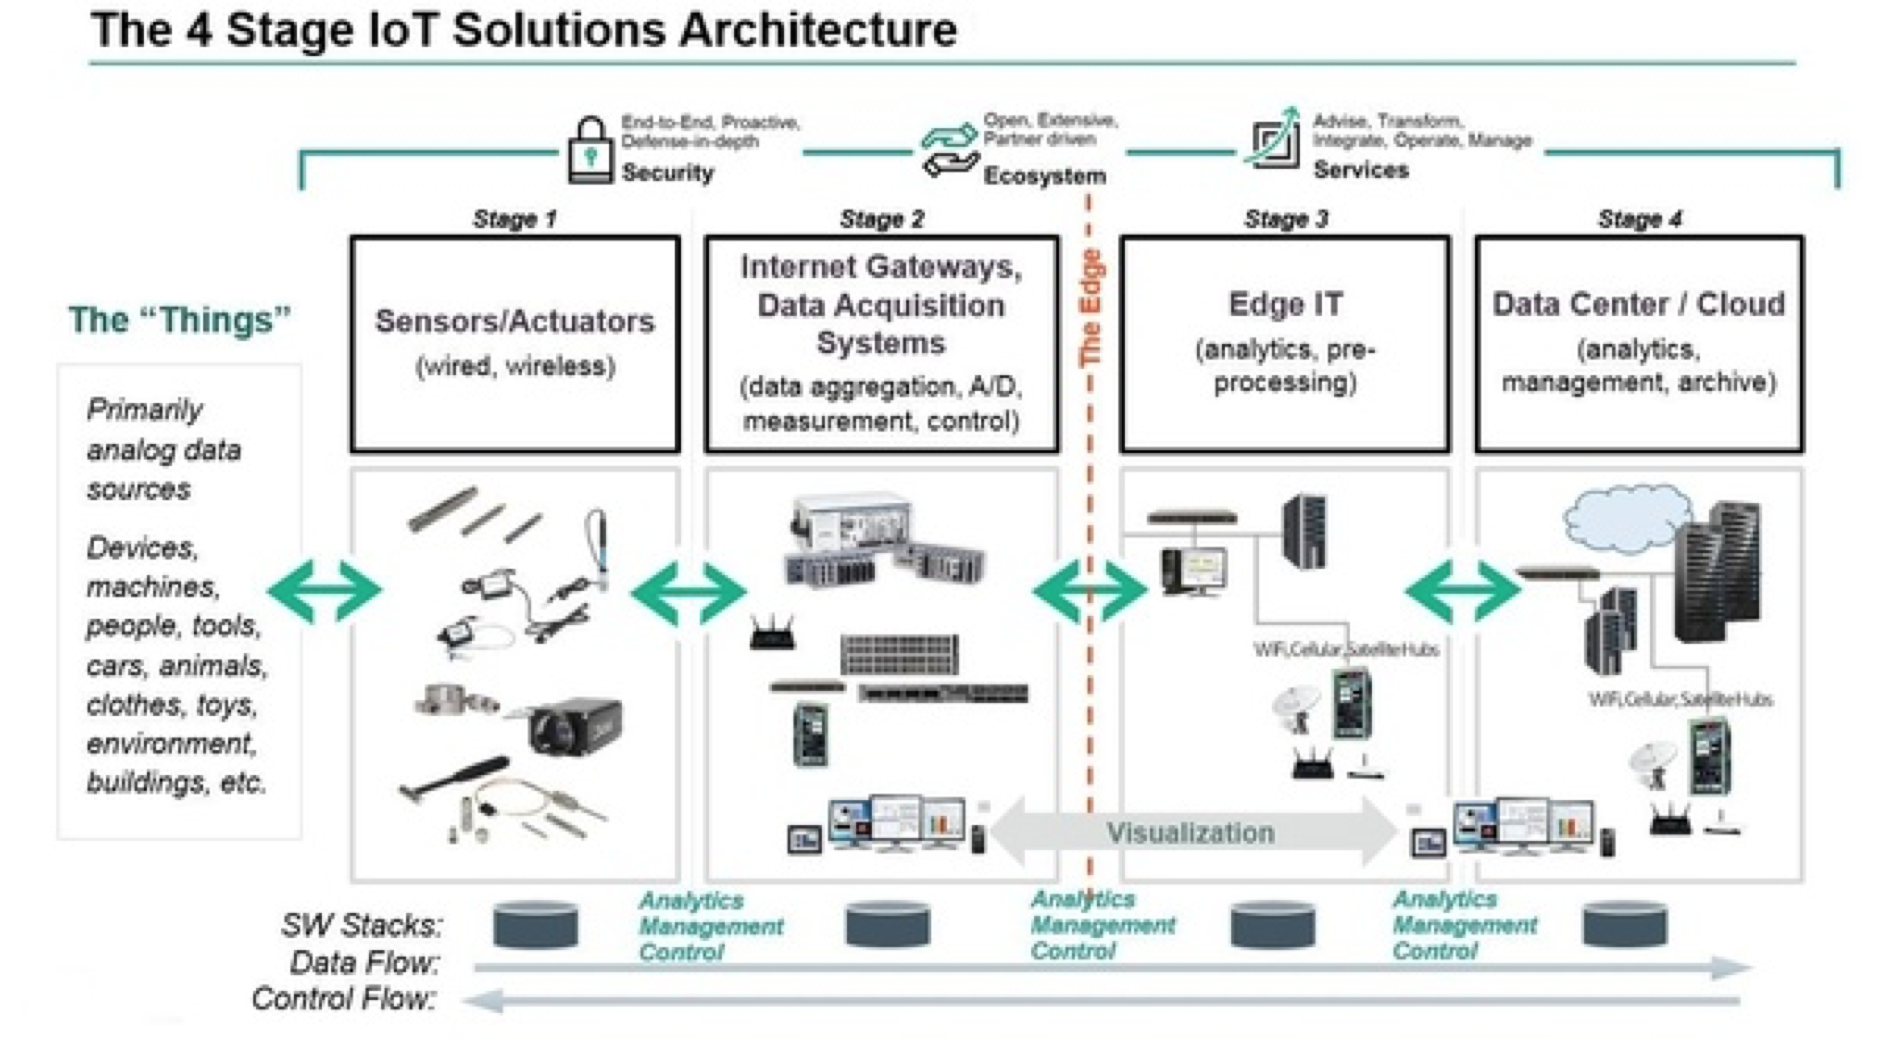
\includegraphics[scale=0.27]{iot-arch}
\centering
\caption{Standard Internet of Things Architecture \protect\cite{stokes}}
\label{fig:iot-arch}
\end{figure}

The IoT system architecture is usually described as a four part process, in which data is collected from endpoints (all kinds of sensors) and after some pre-processing they finally arrive at a data center where it is properly processed, analysed, and stored. We must also take into account that data or instructions can flow in the opposite direction (from the data center to the endpoints) in order to make decisions about actions to take, usually according to the data previously received. Now we will go through each stage, which will also be taken into account when developing this project \cite{digi}\cite{marlabs}:

\begin{itemize}
    \item The first part would consist of the sensors and the actuators. Those will be in charge of collecting the data from whichever object they might be embeeded in, with parameters such as chemical composition, temperature, humidity or more. The actuators will be the ones able to decide and take actions based on the information previously collected by the sensors, like opening or closing the curtains of a room, depending on if the sun is pointing right at the window. 
    \item The second part consists of the Sensor Data Acquisition Systems. These systems will be able to perform tasks such as converting the data into the right format or compressing it to reduce its size.
    \item The third stage would be the pre-processing of the data at the endpoint side. Tools can be used for this stage, like machine learning or some kind of intelligence system able to make some quick decisions without having to wait for the data center to give the instructions. We want to always make sure that the intelligence is close to the endpoints, instead of close to the data center. 
    \item The last part of the architecture will be focused on the analysis, visualisation and storage of the data collected. This will be performed by the data center, which can be in a physical location, or in the cloud. The analysis of the data center will be much deeper than the one in the pre-processing part, as business rules and specific analysis will be taken place there.
    \item Lastly, it is important to mention Data flow and Control flow. These channels describe the direction these aspects of the system are traveling towards. While the data flow travels from the endpoints towards the data center, the control flow will go mainly from the data center towards the endpoints (as it is the data center who can make decisions and communicate them to the rest of the system).
\end{itemize}

\subsubsection{Applications}

Internet of Things' systems have proven to be able to be very important tools within a very wide range of areas in society, going from consumer to industrial and infrastructure applications:

\begin{itemize}
    \item Some of the consumer applications of IoT include everything from home automation systems that monitor lights, temperature, home appliances and even home security to self-driving cars or wearable technology such as fitness trackers that are able to monitor your health just by wearing them, etc.
    \item Industrial applications of IoT have been very beneficial for most of the economic sectors; for example, primary sector activities such as agriculture are being automated and made more efficient, with systems which collect data from the environment (which is similar to what this project is about) and decide on which techniques are more appropriate for the land. The supply chain industry has also been revolutionised, as now it's a lot easier to figure out where the goods are at any point in time, hence being able to make accurate timelines, making the traffic a lot smoother and more efficient \cite{blume}. Other domains of industrial automation where IoT can prove to be very helpful are also Factory Digitalisation, Inventory Management or Safety and Security measures. 
    \item When we want to talk about large-scale infrastructure applications of IoT we must mention the new Smart Cities, with useful integrations of IoT ranging from more efficient public transformation systems (with real-time information on times and routes and an easier ticket purchasing system) to an automated and smart healthcare system (with an IoT system facilitating data collection and thus improving its administration) \cite{chathuranga}. As the challenges for a city might be very different to other cities, IoT can help analysing the specific features of the city and build a better solution for it.
\end{itemize}

\section{Design and Approach}

\subsection{Project structure}

This project will consist on different stages that must be achieved in order to gain the necessary knowledge to develop a product that can be properly applied to a specialist real world application: 
\begin{itemize}
    \item We will first need to understand the IoT system architecture developed in a previous project, which will serve as the foundation for our monitoring system.
    \item We will then need to develop the functionality for this system, focusing on key aspects such as how the data is collected, how this data can be stored, and also how the data can be transferred through the network to the database.
    \item In order to make the system ``smarter'' we will need to focus on making the appropriate decisions in order to maintain the well-being of the system, which is the principal objective of parameter monitoring.
    \item We will also need to focus on enhancing data reporting and visualisation, in order to show the monitoring status of the different devices of the IoT network, and in data logging, important to store data locally (and therefore keeping the last pieces of information collected safe temporarily) for unexpected cases that could arise like loss of power or the impossibility of transferring the data through the network.
\end{itemize}

\subsection{Requirements}

I will now proceed to outline the main requirements for our project. The project should be able to consist of a system with these characteristics, as they will be very important for the successful development of an independently functioning system, able to be used for real world use cases, in order to help the university team without any issues:

\begin{itemize}
    \item The system must be able to run under the University of Manchester Eduroam network, as the server where the data must be stored is also located in the university network.
    \item Its is expected for up to around 100 sensors to be collecting data simultaneously (scalability concerns). While you can connect a single sensor to a microcontroller, it is preferred for multiple sensors to be connected to a single microcontroller, as reducing the number of microcontrollers will also decrease possible failures from the device.
    \item The data should be easily accessed and dislayed in multiple suitable forms of graphs. A data visualisation platform can be used for this purpose. 
    \item Some kind of memory optimisation technique should be used in order to maximise this limited resource. However, we must not lose any information due to the optimisation.
    \item A simple parameter monitoring system must be added, able to make decisions to maintain the well-being of the system with no help from any developer or member of staff, as this must be an automated process running uninterruptedly.
    \item Information must always be stored, the system must be able to keep the information stored in case of unexpected circumstances, such as loss of power or failures in the network.
    \item Only authorised devices must be able to connect to the database and send data.
    \item We must be able to quickly identify each microcontroller in the network, and its configuration information should be sent along with the collected and analysed data.  
    \item Every microcontroller should be able to easily show its monitoring status, so members of staff can easily see the well-being of the device. 
\end{itemize}

\subsection{System Architecture}

\subsubsection{Overview of the system architecture}

This project will consist of one or multiple microcontrollers that will periodically collect data from sensors. Once multiple readings of the data have been collected, the microcontrollers will be in charge of analysing the data, pre-processing it, and sending it to a time series database (InfluxDB). When analysing the data, the microcontrollers will be able to make quick decisions, thanks to their monitoring system, which will check the well-being of the device. The status of the monitoring device will be easily available thanks to an integrated OLED display. The data stored over time at InfluxDB will be easily available for monitoring thanks to the Grafana visualisation platform. In order to avoid possible loss of data, logging will be implemented in various ways, such as the use of flash memory or an external memory card. Here we can have a look at a diagram about the system:

\begin{figure}[h]
\label{fig:system-arch}
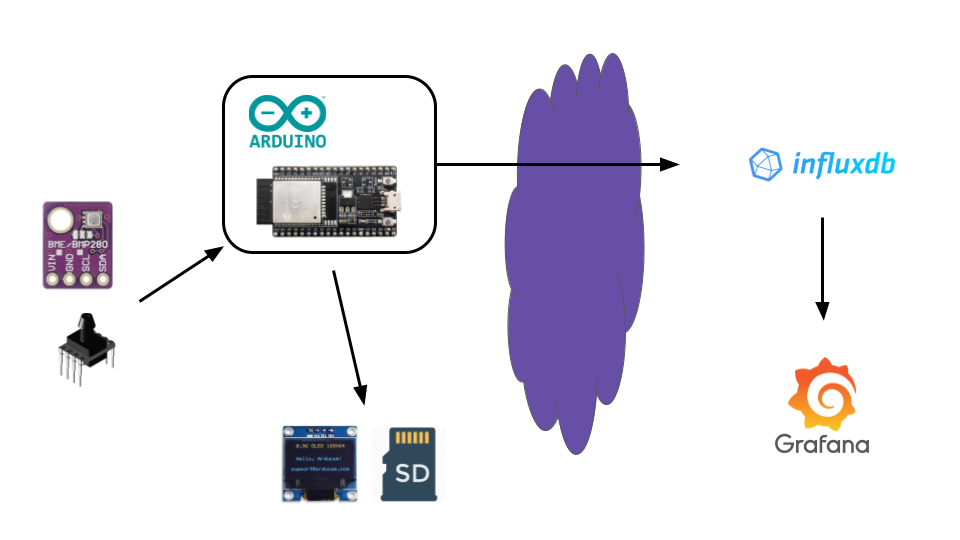
\includegraphics[scale=0.45]{system-arch}
\centering
\caption{Simple diagram describing the system architecture}
\end{figure}

\subsubsection{Hardware components selection}

The decision of the microcontroller board and the other hardware components will be crucial for the best possible and most efficient system. Therefore, we need to be able to define which of them are the most adequate for this project.\par

In the previous project, there were sketches for the use of an Arduino compatible microcontroller board (ESP32) and a DHT22 temperature and humidity sensor. We will consider those choices plus others in the comparison.\par

Choosing the right hardware components for an IoT system is a very important decision to make, as we want to make sure that the different components will be the most useful for our specific needs and that the system will run as efficiently as possible. We must take many factors into consideration, such as scalability, functionality, cost, power requirements, etc \cite{digiteum}.\par

\paragraph*{Microcontroller:}
The most important decision will be choosing the appropriate microcontroller / single-board computer, as this device will power the system and will do most operations with the data. The first important choice was between a microcontroller and a single-board computer (such as a Raspberry Pi). While a Raspberry Pi is more powerful and has its own Operating System, there was no real purpose for its use, as an Arduino microcontroller and its open hardware nature allows for multiple different types of sensors and embedded systems to be connected to the microcontroller thanks to its GPIO pins. We must also take into account that while the microcontroller cannot handle intensive tasks like the Raspberry Pi can, it also uses a lot less power, which is important for this project, as it is running uninterruptedly. Here we can see the different microcontrollers considered in the decision:

\begin{itemize}
    \item The first option considered was the Particle Photon. This microcontroller had a STM32F205RGY6 120Mhz ARM Cortex M3, with 1MB of flash memory and 128KB of RAM. It had 18 mixed-signal GPIO pins and its recommended power supply was from 3.6V to 5.5V.
    \item The second option was the ESP32 microcontroller by Espressif. It was powered by a Tensilica Xtensa Dual-Core 32-bit LX6 microprocessor, running at 160MHz, with 4MB of flash memory and 520 KB of SRAM. It had 34 GPIO pins with multiple functionalities and run with a recommended power supply from 2.3V to 3.6V.
    \item The last option considered was an Arduino UNO WiFi Rev2, with a ATMEGA4809 processor, running at 16MHz. It had 48KB of flash memory, and 6KB of SRAM. It only has 14 GPIO pins and its recommended power supply is from 7V to 12V. 
\end{itemize}

After looking at the different possibilities for a microcontroller board to be used, I have decided that it would be best to go for an ESP32 type microcontroller, because of the following reasons: It has the fastest processor at 160 MHz, better for processing all the information that needs to collect from the sensors; more amount of memory, which will allow it to be faster with more intensive tasks; more GPIO pins available, which will be necessary for the number of sensors that we might need to connect to it and it also has the lowest recommended power supply, which will be beneficial as it will be connected at all times. Apart from all of the previous reasons, it is also the cheapest of all of the options.

\begin{figure}[h]
\label{fig:esp32}
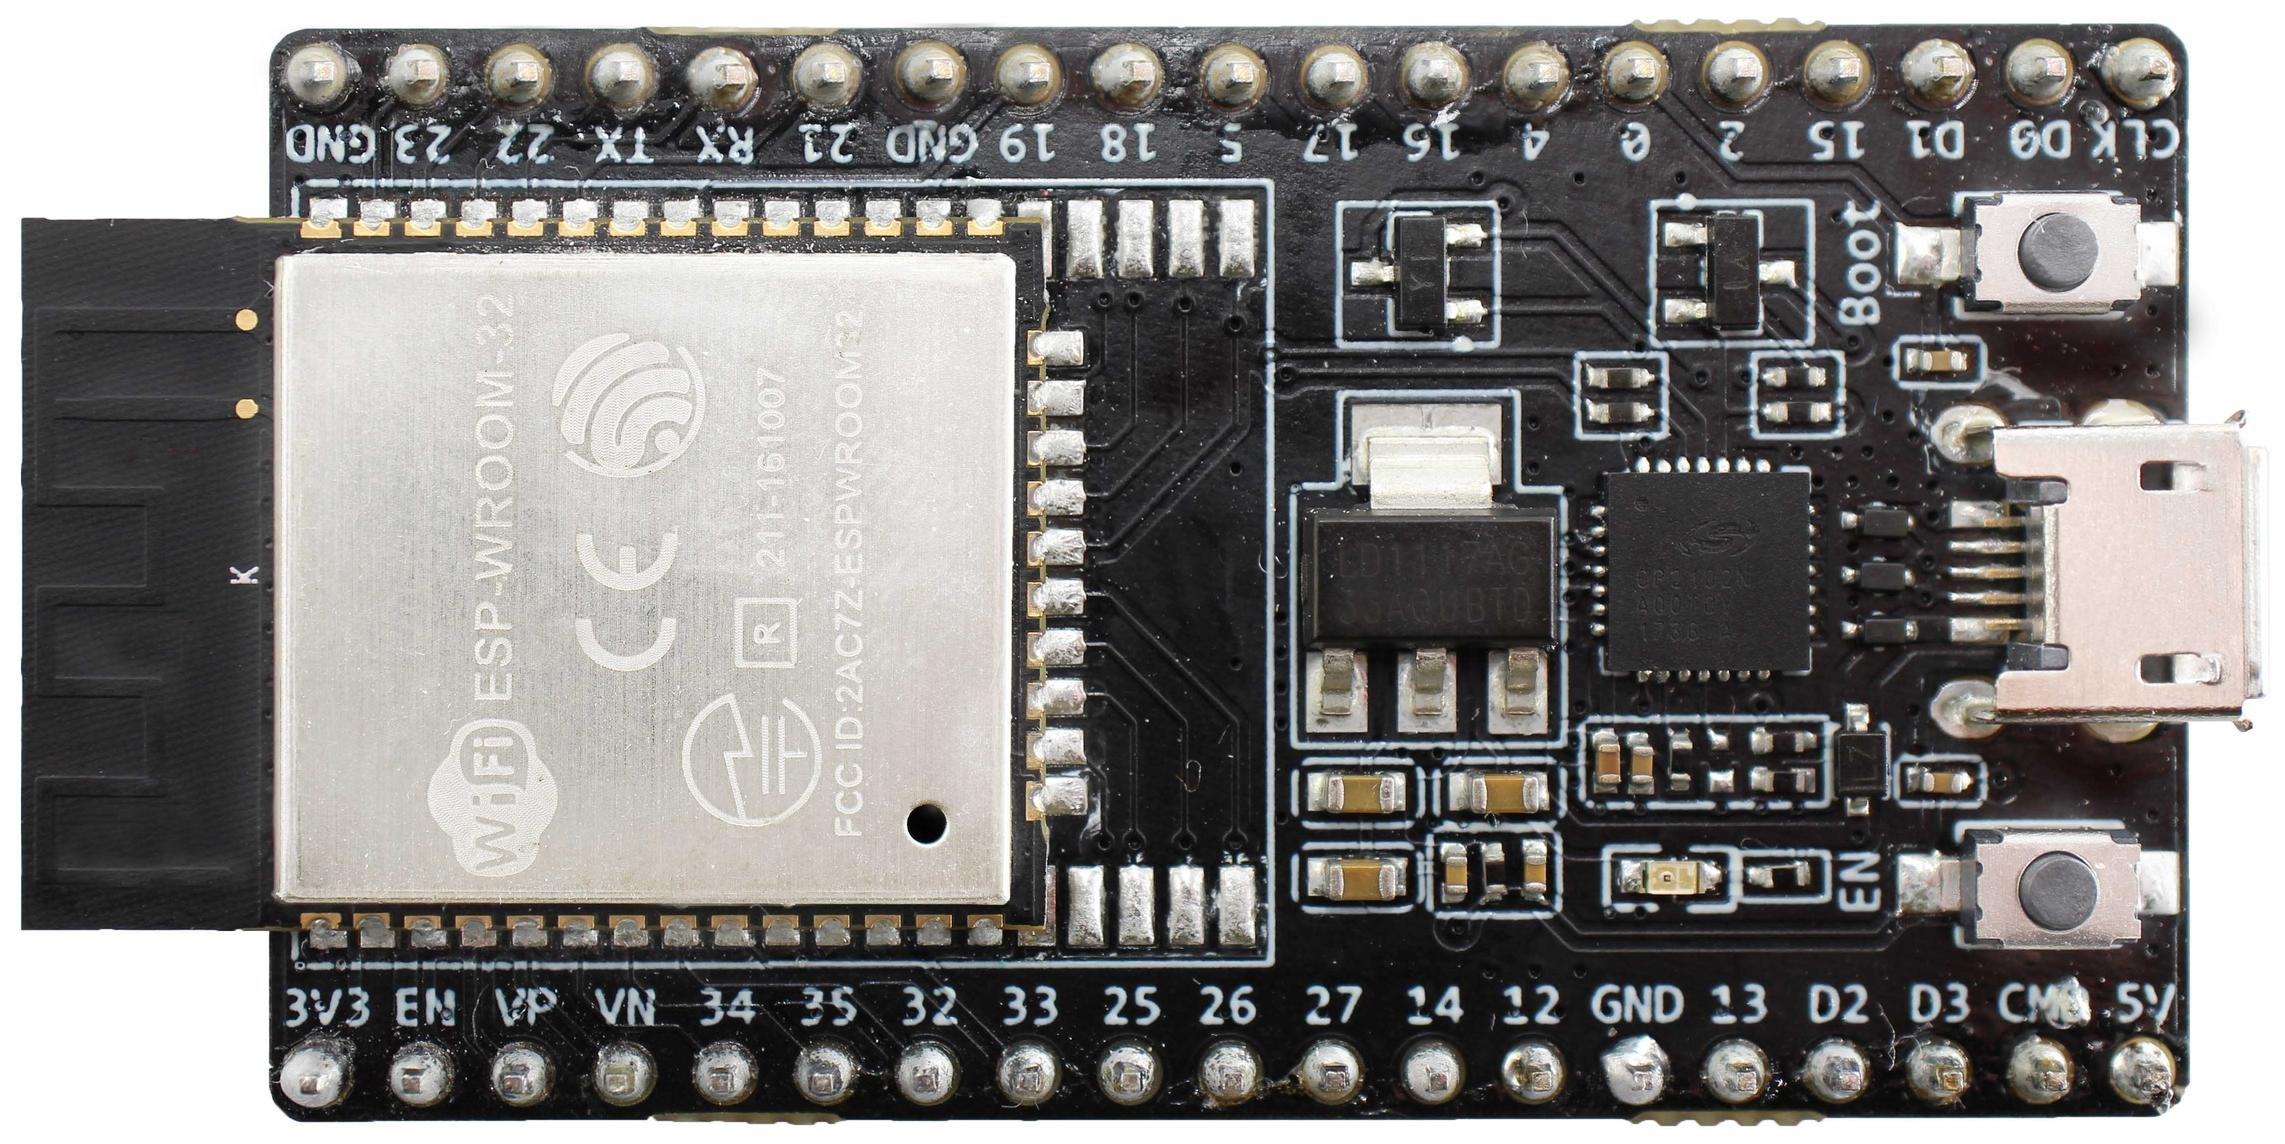
\includegraphics[scale=0.06]{esp32-devkitc-v4-front}
\centering
\caption{ESP32 microcontroller by Espressif}
\end{figure}

\paragraph*{Sensors:}
In this system, we will need to collect basic data for the management of the environment of a cleanroom. Those would be: Temperature, humidity, absolute pressure, barometric pressure. Most of the temperature sensors in this comparison are also able to measure other features such as humidity or even barometric pressure. We will take that into account when comparison. The different options considered for the temperature and humidity sensors are:

\begin{itemize}
    \item The first option is the DHT22 temperature and humidity sensor. This was the sensor chosen in the previous version of this project. It measures temperature from -40C to 80C, with an accuracy of +-0.5C, and it covers from 0\% to 100\% of humidity with an accuracy of +-2\%, with its recommended power supply from 3V to 6V. However it does not measure barometric pressure, which might be useful in terms of using as least hardware as possible.
    \item The next option is the LM35DZ temperature sensor. It measures temperature from -55C to 150C, with an estimated accuracy of +-0.5C at 25C, with its recommended power supply from 4V to 30V. However it does not measure humidity or barometric pressure.
    \item The last option is the BME280 temperature, humidity and barometric pressure sensor. It measures temperature from -40C to 85C, with an accuracy of +-0.5C, and it covers from 0\% to 100\% of humidity with an accuracy of +-3\%, with its recommended power supply from 3.3V to 5V. It also measures barometric pressure sensor, from 330hPa to 1100hPa, with an accuracy of +-1hPa.
\end{itemize}

After looking at these three main possibilities, I decided to go for the BME280, because I found it easier to find, and cheaper. This was my line of thoughts: I ruled out the LM35DZ because it did not have a humidity sensor as well as the temperature sensor, so it meant to look for a different sensor for the humidity. Most of the humidity sensors came in conjunction with a temperature sensor so it was not a good choice. Also, it was analogue, so it would use more power, needing more power supply for it. I decided to go for the BME280 because it was easier to find and cheaper, apart from also being able to measure barometric pressure.\par

\begin{figure}[h]
\label{fig:bme280}
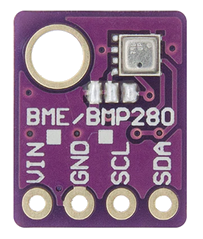
\includegraphics[scale=0.25]{BMX280}
\centering
\caption{BME280 temperature, humidity and barometric pressure sensor}
\end{figure}

We will next look at the absolute pressure sensors, also called pressure transducers. At the beginning of the search I found some options that I thought could be valid for our project (such as the MPXH6400AC6U, MPXA4250AC6U and the MPX5100AP). However, these all could only measure from 0kPa to 400kPa approximately. After learning that we were looking for a sensor with an operating pressure range of 0bar to 10bar, I had to start searching again. I could only find one model able to operate within that pressure range, the Honeywell HSCDLNN010BASA3 (010BASA3 for short). Due to various factors (including Covid-19 restrictions) the sensor did not arrive, and I was instead delivered a differential pressure sensor (010BGAA5). Due to the fact that we were not going to the CMN facilities at all (because of the pandemic) and both are analog sensors that connect to the microcontroller in an identical way, I decided to use that sensor (even if it was not what I originally wanted). This change does not affect the outcome of the project in any way, so there are no problems with this decision.

\begin{figure}[h]
\label{fig:010BGAA5}
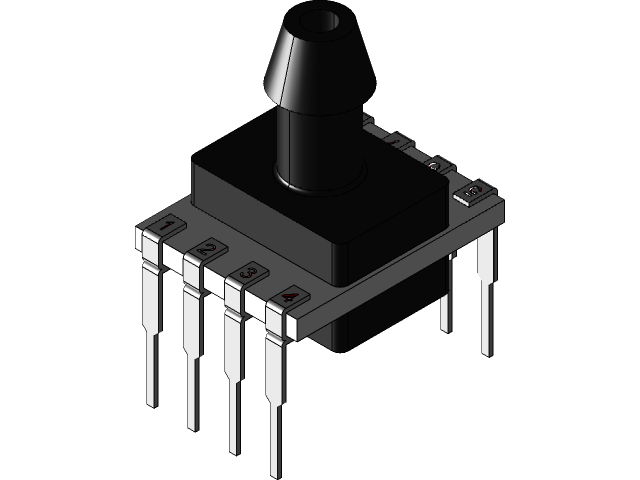
\includegraphics[scale=0.15]{large}
\centering
\caption{Regular analog pressure tranducer}
\end{figure}

\subsubsection{Storing Time-Series Data: InfluxDB}

We call Time Series Data to ``the collection of data through repeated measurements over time''. This means that we will get a sequence of data points that will be organised by the time they were measured at. The purpose of the collection of this type of data is mainly to monitor certain parameters closely and easily detect any change that may occur \cite{influx:time-series}.\par

In this project we will be storing time series data in the form of temperature, humidity, barometric pressure and differential pressure readings. Because of this we have to choose the most appropriate database for this purpose. The database selected for this project was InfluxDB, a time series database designed for fast and high availability storage and retrieval of time series data. Time series data is stored by InfluxDB in a way that each field contains a series of blocks of time which are stored contiguously on disk, therefore being very optimised for fast operations on the data. Apart from that, InfluxDB uses a Line Protocol when sending time series data, which easily provides the query with the measurement, tags, fields and timestamp for very fast lookups \cite{influx:time-series}. It also offers clear advantages in speed when storing and indexing time-stamped data. This is because while other traditional databases would slow down when organising complex indices, InfluxDB is able to maintain high indexing speed because it uses a much more simple indexing system \cite{ionos}. \par

\begin{figure}[h]
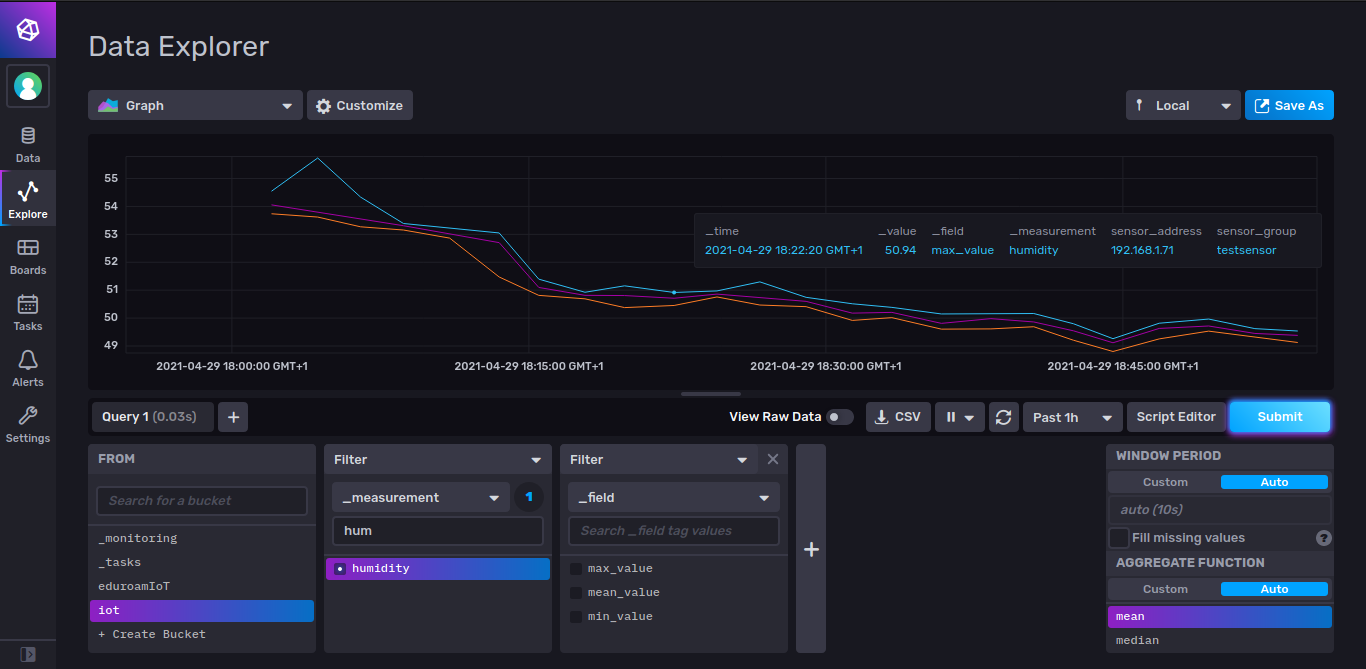
\includegraphics[scale=0.35]{influx-dashboard}
\centering
\caption{InfluxDB's dashboard (Option to filter by measurement name or other parameters)}
\label{fig:influx-dashboard}
\end{figure}

The structure of the data points stored in InfluxDB is very simple. At the highest level we have the name of the measurement. This will then be followed by two main key value pairs called the tags and the fields. These tags describe the metadata, while the fields will contain the actual values of the measurement that are to be analysed and stored. All of this will be accompanied by the time stamp of the data point. \par

One of the most important features of InfluxDB specific for this project is its schemaless design, as it allows for a better management of discontinuous data. This means that if some of the data does not appear in a few readings, this does not result into a problem with parsing and transferring to InfluxDB.\par 

InfluxDB is also very easy to work with and implement because it has no external dependencies, making it a lot easier to run, and also contains very high performing HTTP APIs, which will make the data transfer using these APIs a lot easier. It also has a sample client available, so it becomes very fast and easy to start for beginners or new developers interested in this database.

\subsubsection{Data visualisation: Grafana}

Grafana is one of the most important data visualisation platforms, as it provides an extensive range of functionalities and it is very easy to use and manage. We will explore its different advantages and features in order to gain a basic understanding of the purpose of this data visualisation platform.\par

\begin{figure}[h]
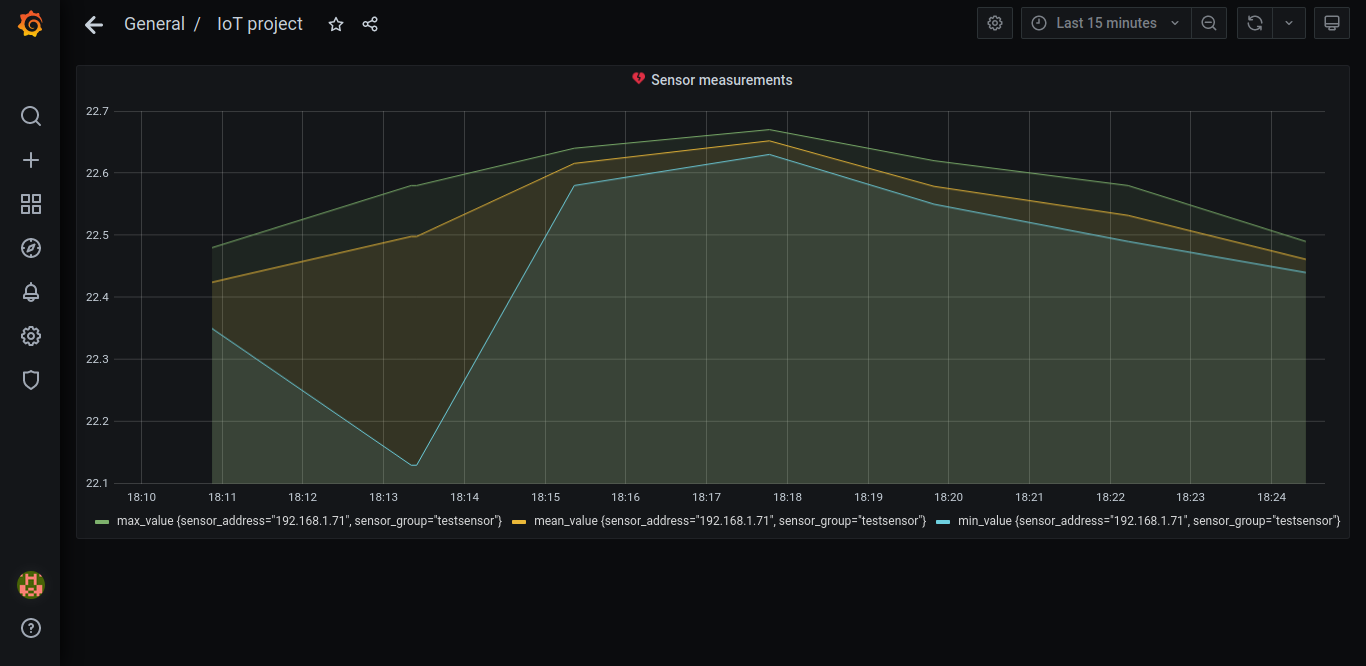
\includegraphics[scale=0.3]{grafana-dashboard}
\centering
\caption{Simple view of the Grafana dashboard, where humidity values are being queried}
\label{fig:grafana-dashboard}
\end{figure}

Even if InfluxDB has its own dashboard in which you can keep track of the data, using Grafana also allowed us to introduce an extra layer of monitoring (this time from the server side), thanks to its Alerting feature. Grafana's alerting feature allows to send messages in many different ways (Discord, Teams or Slack notifications, e-mails, HTTP POST requests to specific URLs, etc.) according to the data collected. This can easily be done by everyone thanks to its graphical user interface, as you can define ranges of values allowed or conditions to be met interactively, without any need of programming knowldege \cite{grafana}. As this feature would be focused more on the backend/server side of this IoT system, it will be futher explored by my partner, in his counterpart of the project.

\begin{figure}[h]
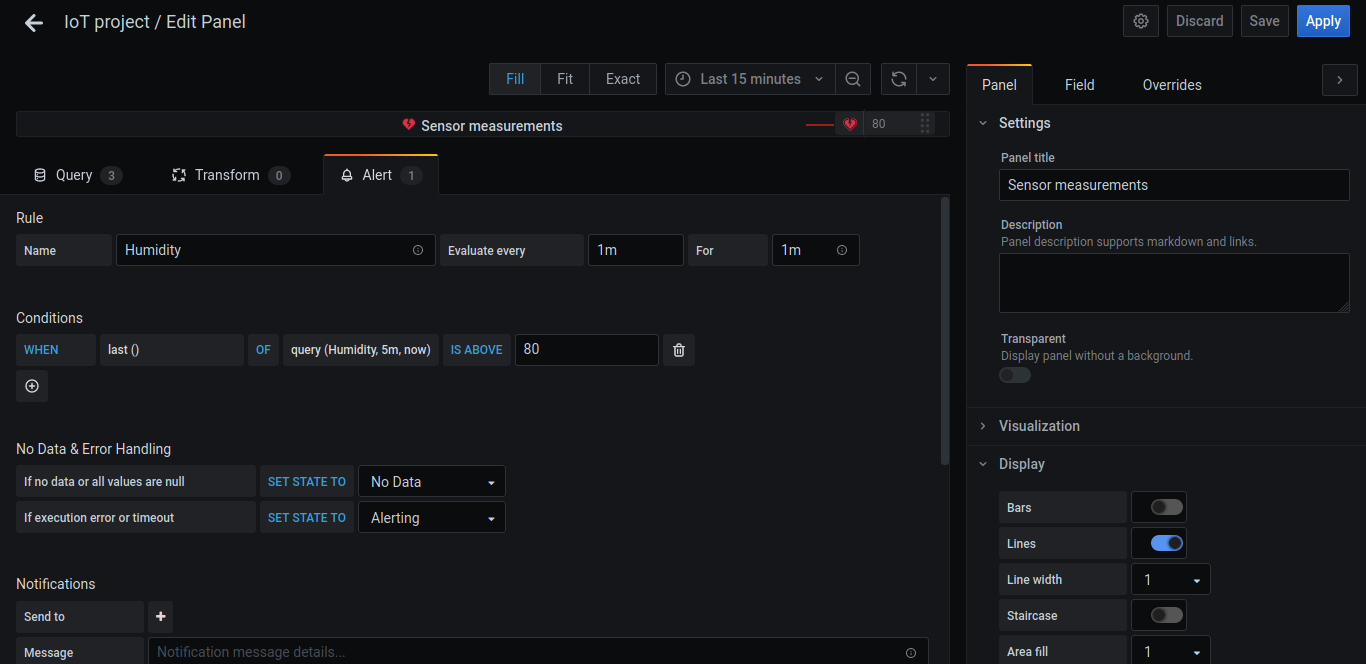
\includegraphics[scale=0.3]{grafana-alerting}
\centering
\caption{Grafana's alerting functionality}
\label{fig:grafana-alerting}
\end{figure}

Grafana also has a wide variety of dashboards, such as heatmaps, histograms, geomaps, etc. This is also very useful, as it provides with different ways of displaying data, such that we can use different ones according to the data received, making it a lot more comfortable to use and easier to visualise.\par

Finally, Grafana is also able to provide support for many data sources, so we are not only able to import data from InfluxDB, but also from many others such as Graphite or Prometheus. This is a really interesting feature in terms of future scalability of the project, as the possibility of integrating many different data sources will be really useful for different types of data.

\subsubsection{Security and Authentication: Tokens}

This system is meant to be running in the University of Manchester Eduroam network, within the Manchester CMN server. Eduroam is a world-wide roaming service for the research and education community. It allows students and staff to connect to the Internet in an easy and secure way. This WPA2 Enterprise network uses the IEEE 802.1X standard for port-based Network Access Control, providing authentication of users in order for only authorised users to access the data shared over the network. Thanks to this, most of the security breaches are prevented, as only known users with access to the network would be able to access the data \cite{eduroam}. \par 

However, this does not mean that all security threats are prevented, as users authorised by the network could still attack the system. In order to ensure the interaction between different users and the database in a secure way, InfluxDB uses a token authentiation system. A specific token belongs to a user/organization that interacts with the database. This token is also able to reflect their InfluxDB permissions.\par

There are three types of tokens: Admin tokens, All-Access Tokens and Read/Write Tokens. Admin tokens cannot be created manually, and have full access to all the different organisations in the database, with both read and right permissions to every single resource in each organisation. All-Access Tokens have full read and write access to every resource in a single specific organisation, while Read/Write Tokens have access to some specific resources in an organisation. In order to avoid possible mistakes when handling multiple organisations, it is more preferable to create an All-Access Token for every single organisation, rather than using the same Admin token for all of them \cite{influx:tokens}.\par

Thanks to Grafana's Alerting feature, it is possible to remotely use the network to send HTTP requests that could remotely change things such as the sensor configuration parameters and more. In order to carry this new functionality out (which is being explored by my project partner in his counterpart of the project) the Arduino would need to host a HTTP server. However, this would mean that new possible security threats would appear, in which authorised Eduroam users could change the sensor configuration through an HTTP request. In order to prevent this, authentiation to the HTTP server should be necessary and would need to be implemented.

\section{Implementation}

Having chosen the appropriate hardware that will be used in order to carry out this project, I will now start talking about the different stages of the implementation, along with the specific areas of interest in which different tasks were performed in order to develop this IoT system. 

\subsection{Data collection}

The first area of focus of the project is the collection of data. In this stage we will focus on how to collect the data from the sensors, in order to analyse it and pre-process it.\par

First, we will talk about the ESP32 microcontroller GPIO pin system. The ESP32 microcontroller has 48 pins, with multiple different functionalities such as Analog to Digital (ADC) channels, Digital to Analog (DAC) channels, UART, PWM, I2C and SPI communications, capacitive sensing pins, etc. Some pins have functions assigned by default, but most of them can be changed in the code. This is thanks to the ESP32 multiplexing feature (multiple peripherals connected to a single GPIO pin) \cite{randomnerd:gpio}. In order to talk about how the different hardware components were integrated into the system it is important to understand the types of communication protocols they use to interact with the microcontroller, the I2C and SPI protocols.

\begin{itemize}
    \item I2C is a serial communication bus (sends data 1 bit at a time), used for peripherals without a focus on speed, but rather on low manufacturing costs and simplicity. With I2C you can have one or more master devices controlling one or multiple slaves, therefore it is very useful when performing multiple tasks with a single microcontroller, which is our specific case. It consists of two main lines which contain the data to be transmitted between the master and the slaves (SDA) and a clock signal (SCL), which is shared between the devices. I2C is synchronous, therefore the output is synchronised to the clock signal, which is controlled by the master. However, data is sent in packets, with a limited number of bits, therefore interrupting the transmission between each packet.
    \item SPI is a synchronous serial communication interface, which supports a single master controlling one or multiple slaves. SPI is also known as ``the 4 wire bus'' due to the fact that consists of 4 four wires: MOSI, MISO, SCLK and CS. MOSI stands for Master Output Slave Input, line used for the data sent from the master to the slave. MISO (Master Input Slave Output) is the line which does the opposite, sending data from the slave to the master. SCLK is the clock signal, used in the same way as I2C, as it is also a synchronous communication bus. Lastly, the CS (Chip Select) line will identify which slave the master is interacting with. Differently to the I2C bus, the stream of data does not need to be interrupted during transmission, as any number of bits can be sent continuously.
\end{itemize}

\subsubsection{Integrating the BME 280 sensor}

The specific version of the BME280 sensor is able to support both I2C and SPI communication. In this project it will be connected to the microcontroller using I2C communication. In the ESP32 microcontroller, the default pins for I2C (and the ones we are going to use for this project) are GPIO 21 (SDA) and 22 (SCL). We will also connect the Vin (Voltage input) line to the 3.3V pin and the Ground line (GND) to the Ground GPIO.\par

In order to easily integrate the sensor with the microcontroller, it is necessary to download and import two essential external libraries specific for the sensor: The Adafruit BME280 library and the Adafruit Unified Sensor library. These are made by the manufacturer in order to easily program the sensor. After this, we just need to include the appropriate code:

\begin{figure}[h]
\label{code:bme}
\lstinputlisting[language=C++]{bme.ino}
\centering
\caption{Sample code for integrating the BME280 sensor}
\end{figure}

\subsubsection{Integrating the Honeywell 010BDAA5 sensor}

The Honeywell differential pressure sensor will be a lot simpler to integrate, as it is an analog sensor. This analog sensor only has 3 wires: Ground (GND), which is the line that will connect to the ESP32 GND pin, Voltage Input (3.3V), which is the higher voltage with respect to GND, and Voltage Output (Vout) which will contain the measurement and will connect the any Analog to Digital input GPIO. When reading an analog sensor, you are measuring voltage levels between 0V and 3.3V. The voltage measured will correspond to a value between 0 and 4095, as these analog pins have a 12-bit resolution. However, we must take into account the fact that ADC channels are not linear, so the ESP32 microcontroller will not be able to recognise properly the the highest or lowest voltages, giving the same result for voltages close to each other in these ranges.\par

For this project I decided to use GPIO 34 as the pin where the Voltage Output line will connect to. Now the next step is to read the value measured by the sensor and convert it according to the specifications of the piece of hardware. In this case, the range of the sensor is from 0 bar to 10 bar, so the value measured will be converted to a final value within the sensor range.

\subsubsection{Integrating the Velleman VMA438 OLED display}

The Velleman VMA438 OLED display will be connected in a similar way to the BME280 sensor, as it also uses I2C communication. As mentioned before, I2C provides support for many slaves to be controlled by a single master device, so we are able to use the same pins for SDA (21) and SCL (22).\par

In order to integrate this display, it is necessary to use its external library, U8g2lib. It provides specific methods that will set up the font, text position, etc. as well as very useful methods for drawing a wide variety of shapes.

\begin{figure}[h]
\label{code:oled}
\lstinputlisting[language=C++]{oled.ino}
\centering
\caption{Sample code for integrating the VMA438 OLED display}
\end{figure}

\subsubsection{Integrating the microSD card adapter}

The HW-125 microSD card adapter uses SPI communication in order to connect to the ESP32 microcontroller, therefore this time we will use different GPIO pins to the ones we used for I2C communication. The MOSI line will connect to GPIO 23, the MISO lie will connect to GPIO 19, the SCLK (Serial Clock) line will connect to GPIO 18 and the CS (Chip Select) line will connect to GPIO 5.

\begin{figure}[h]
\label{code:sd}
\lstinputlisting[language=C++]{sd.ino}
\centering
\caption{Sample code for integrating the HW-125 microSD card adapter}
\end{figure}

\subsection{Memory usage}

One of the biggest challenges of working with one of these Arduino compatible microcontrollers is the appropriate use of its memory, as it is a limited resource that can be very useful, specially for our project. In order to try and store as much information as possible in the limited space that I have, I needed to reduce the size of the information as much as I could.\par

The raw data that is collected from the sensors is not immediately sent to InfluxDB. Instead I decided to collect various readings from the sensors over a defined period of time. Once I have collected enough readings, I obtain their statistics (I calculate the minimum value, mean value and maximum value) and then proceed to send those through the network to InfluxDB.\par 

In order to easily explain how the memory optimisation will be I will first have to explain how the data is constructed when sending it to InfluxDB: When we send data to InfluxDB, we effectively want to create a Datapoint, which is a data structure able to be represented by a string by being formatted in a specific way. This Datapoint will be formed by a series of data structures called KeyValue pairs. These key value pairs will be formatted as strings in the format [key + ``='' + value]. Examples of these data structures are ``sensor\_address=198.162.0.3'' or ``temperature=28.75''. These key value pairs can be divided into 2 groups, tags and values. Tags are those key value pairs that hold the information about each specific microcontroller, such as the sensor address or the sensor group. The tags will help identify each microcontroller and monitor each one of them specifically. Values will hold information about the data that we want to monitor, such as the mean value, maximum value or even the different sensor configurations like the time of every push interval, etc. The format of the Datapoint will then be as follows: [measurement\_name, tags values] where each key value pair in both tags and values will be separated to the next by a comma (,) (Example: ``humidity,sensor\_address=198.162.0.3,sensor\_group=3 min\_value=45.56,mean\_value=47.84,max\_value=48.54'').\par

Once the data has been pre-processed and the Datapoints have been created, they must be stored in a buffer. Every certain amount of time, this buffer will be flushed and sent to InfluxDB. However, not all HTTP requests will succeed and go as planned, and therefore we must account for the times when the network will not be functioning properly. When this happens, we do not want to lose the information, as it can be very valuable. Because of this, we want to keep the information stored locally in the buffer, so when the HTTP requests all work again, all the stored metrics would be sent to InfluxDB (If this happens, all those metrics will appear to have been collected at the same time, as the timestamp is created once they reach InfluxDB. This will be futher explored in the later sections of the project, where we will discuss different data logging options).\par

In order not to lose the data, we need to keep as much information in the buffer as possible, so every small optimisation of that Datapoint would be a big advantage. As this project is about real time data collection, it consists of collecting the same metric periodically over a period of time. This means that over the course of many readings, the buffer that contains those Datapoints ends up storing the same information about the sensor and measurement type many times. That ends up being a lot of wasted storage that could be used in storing more metrics. In order to do that, I chose to implement bidirectional mapping: \par

\begin{figure}[h]
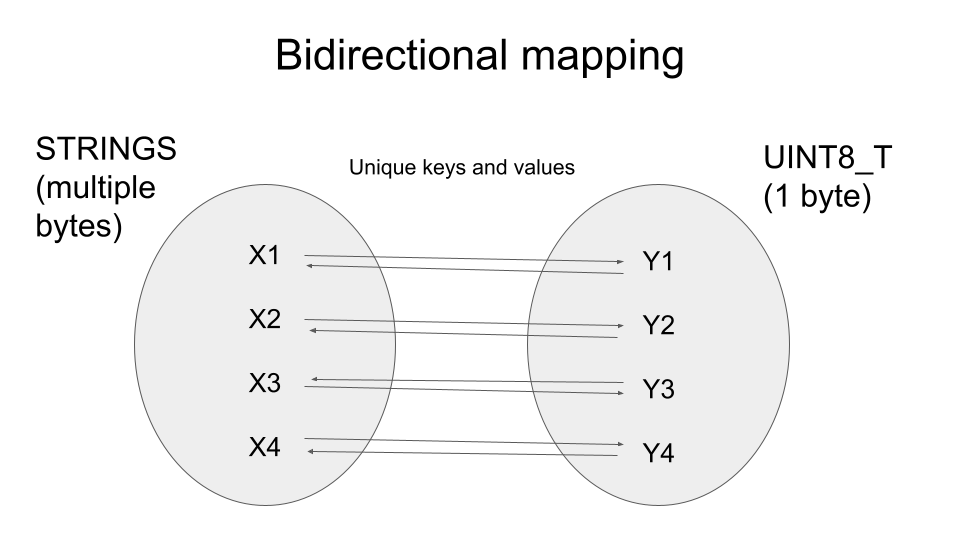
\includegraphics[scale=0.4]{Bimap-diagram}
\centering
\caption{Simple diagram of a bidirectional map}
\label{fig:bimaps}
\end{figure}

\begin{itemize}
    \item I initialise the map with some strings that I know will appear many times over the collection of readings, such as strings about the tags (sensor configuration) or about the statistics of the data (minimum/maximum value, etc.). I assign to these strings the first few numbers starting from 0. The measurement names (such as ``temperature'') will be added by the developer when uploading the new microcontroller code, and they will be assigned to the next numbers in order until 255.
    \item Instead of storing these strings (like ``humidity'', ``max\_value'' or ``sensor\_address'') every time a new Datapoint gets added, I will only store the associated number. 
    \item By implementing bidirectional mapping, we can make sure that there are unique keys and unique values, and therefore we will never have problems associating a specific byte to a specific string.
    \item While there is an implementation of bidirectional maps in the Boost external library, it had many functionalities that we were never going to use. I found a lot easier and memory effective to implement two symmetric maps; while we had to store the mapping twice over the course of many readings, this method proved to be very memory efficient. 
\end{itemize}

This implementation will not only be useful for buffer storage optimisation, but it will also provide with a way of identifying the measurements, as we will now have a measurement ID that we can use in situations like data logging (This will be explored in a later section).

\subsection{Monitoring system}

\subsubsection{Monitoring status and Alert levels}

\begin{figure}[h]
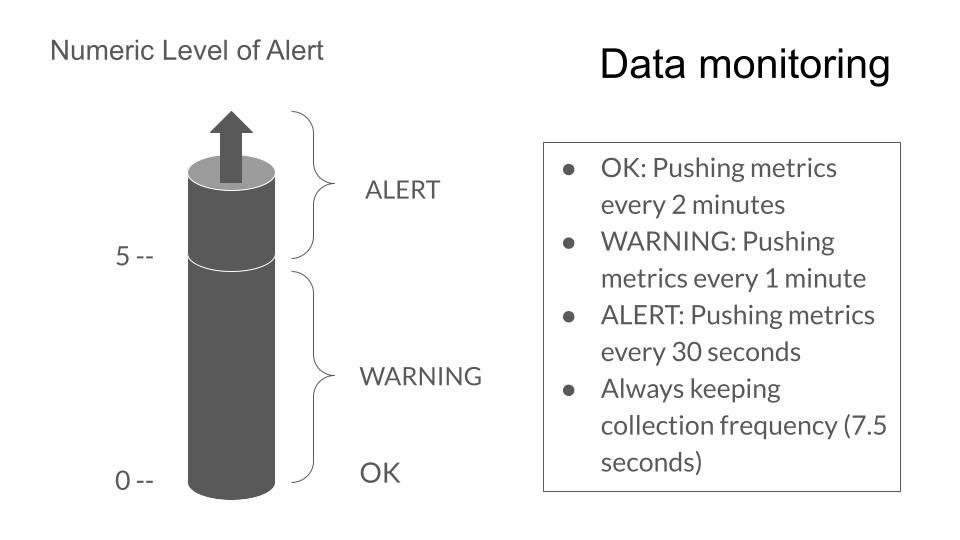
\includegraphics[scale=0.35]{monitoring}
\centering
\caption{Simple diagram explaining the monitoring status and the numeric level of alert}
\label{fig:monitoring}
\end{figure}

In order to add a level of intelligence to the Arduino ESP32 microcontrollers, I chose to introduce a basic monitoring system, which would be in charge of making different decisions according to the data that it is being collected. With this system in place, the microcontroller would be able to change vital parameters of the system such as the time it takes to send a group of measurements to InfluxDB. As mentioned before, the intelligence system should be as close to where the data is collected as possible. This is because we want to be able to quickly make decisions, ideally without having to go through data transfers through the network, where many different problems can arise. Instead, if the microcontroller that collects the data from the sensors is able to take some of the load from the server and already make decisions that can prevent problems with the system,the overall flow of the system will be a lot smoother and less prone to errors.\par

The monitoring system consists of three main possible status, called ``OK\_'', ``WARNING'' and ``ALERT''. These will represent what we will call the ``health of the data''. This basically means that they will reflect if the data that is being collected from the sensors is within the bounds that we should be expecting them to fall into or not. We will be able to define those upper and lower thresholds before compilation, so if some data is falling outside of the range within the thresholds, we will note it as a possible error or failure in the health of the data. Depending on which status the ESP32 microcontroller is in, the frequency of pushing the data to InfluxDB will vary. The monitoring status of the system will be updated every time data is sent to InfluxDB, as it is then when the data is pre-processed, grouped, and analysed.\par

In order to appropriately change between status, I had to come up with a design that would specify when exactly the best time is to change monitoring status, with everything that this change could entail. That is why I decided to use a variable called ``warningToAlert''. This variable will contain a number that will act as the measurement for how far up the alert scale we are right now. When the device is ``OK\_'', this variable will be set to 0. This will be its minimum value. \par

This is how the data collection frequency will vary, according to the design of my monitoring system: 
\begin{itemize}
    \item OK\_: This status will indicate that everything is going as expected, with all values falling within the range defined by the developer. At the moment, the InfluxDB push interval is 120 seconds. This was chosen to be the default value for data transfers, as it allows for multiple readings to be taken before the average, minimum and maximum values are sent through. I also chose 16 as the default number of readings per metric sent, giving a frequency for data collection of 7.5 seconds. I chose 16 because it was a power of 2, so it was easily doubled or halved according to the status of the device. It also means that a large number of values are being collected before sending the data, and hence following the guideline of ``collecting as much data as possible and maintaining the system with the least amount of data transfers through the network as possible''.
    \item WARNING: This status will indicate that some data might not be falling within the range of expected values that we defined, but this has happened recently and should not be taken as serious as the final status. When the device is in a WARNING status, the push interval to InfluxDB is lowered to 60 seconds, while the amount of readings per metric is lowered down to 8. By doing this, we keep the same frequency for the data collection from the sensors but we monitor the system more closely, as we send data to InfluxDB more often. If the device is ``OK\_'' but a single measure does not fall within the thresholds, it immediately goes into the ``WARNING'' status, but the numeric level of alert (reflected by the variable warningToAlert) becomes 2, so the numeric level must go down to 0 by sending 2 sets of ``healthy'' measurements to InfluxDB. I decided against increasing the numeric alert level by just 1 if the monitoring status is OK\_ because I feel that we should make sure that this is under control, and we must be very careful in order to prevent problems with the environment. Once the monitoring status is WARNING or ALERT, the numeric level of alert will only increase by 1 if a set of ``unhealthy'' data is detected.
    \item ALERT: This status reflects that there have been multiple unhealthy measurements collected over the last period of time, and they should be taken seriously and tried to be fixed. This monitoring status is reached when the numeric level of alert reaches 5. The push interval to the database is further lowered to 30 seconds, and the readings per metric get lowered to just 4 (keeping the same data collection frequency of 7.5 seconds). 
\end{itemize}

This system has proven to be an efficient way of monitoring the health of the data, with the objective of sending measurements more often to InfluxDB if the data that was being collected was not being expected. This point is the furthest the Arduino microcontroller will go to, as the server side (which was explored in more depth in the other counterpart of this project) consisting of InfluxDB and Grafana (or even a sensor control service application) will then have the possibility of create different types of alerts (such as email notifications) to quickly inform the appropriate members of staff.

\subsubsection{Extra visual monitoring: Velleman VMA438}

After adding this system, we still needed an easy way to check the health of the data collected by the device. Even though we could do that by going to either the InfluxDB or the Grafana dashboards, I wanted to make it easier to the members of staff already present by adding another piece of hardware to each microcontroller, a 128x64 OLED display. I decided to purchase the Velleman VMA438 OLED display, that connects to the Arduino via the I2C protocol. The display was easy enough to integrate, thanks to the external library U8g2lib that could be downloaded from the manufacturer's website. This library was really easy to use, and provided many different drawing functionalities that made it a great purchase, even if we did not need to use all of its capabilities. Any 128x64 OLED display with I2C protocol would have worked as well, as there are several libraries by Adafruit that easily integrate them with the microcontroller, but I found that the VMA438 would not work seamlessly with those libraries. If the VMA438 is not purchased, the code that integrates the display with the microcontroller would need to be changed. However, I am happy with my decision as it served its purpose, which is to display the monitoring status of the device at all times, letting the staff know if there is something that should be looked further or not.

\subsection{Data Logging}

\subsubsection{Flash memory: Status bytes}

In order to add an extra level of monitoring to the Arduino in unexpected conditions (such as loss of power) I needed to make sure that the latest information collected by the Arduino would be stored in flash memory (so when the power goes back on, the information should still be there). However, as mentioned before, memory is a limited resource so I wanted to store as much information as possible in the least amount of memory as possible. After some research and discussions, I came across the concept of ``status bytes'', and decided to further investigate on them. An example of where status bytes can be found are MIDI (Musical Instrument Digital Interface) messages, where the status byte (which is the first byte in a message) represents the type of action that should be performed \cite{recording-blogs} \cite{midi}. \par 

After discovering how much information a single byte could be carrying I decided to implement this system and store the last readings in flash memory, so if there was ever the need to check the microcontroller in order to see what had been happening with the readings until now, we just had to look at the status bytes last stored. These bytes can easily be checked by using the simple program I implemented called the ``Maintenance Interrogation'' program. \par 

\begin{figure}[h]
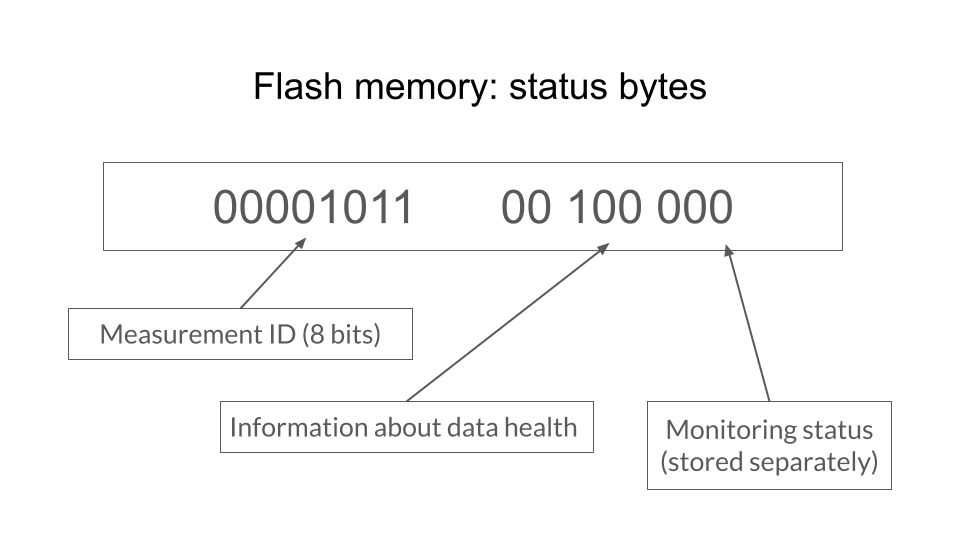
\includegraphics[scale=0.35]{status-byte-info}
\centering
\caption{Information stored in a status byte reading}
\label{fig:status-byte-info}
\end{figure}

For every measurement analysed and sent to InfluxDB a status byte would be stored in memory, describing if the value had fallen within the range defined by the thresholds, if it was higher than the upper threshold or lower than the lower threshold. After every measurement was analysed, a final status byte with the new monitoring status would also be stored. However, 1 byte was not enough to describe all the information, so instead I decided to use 2 bytes for the status:
\begin{itemize}
    \item The first byte would correspond to the binary value associated to each measurement name. This value is reused from the buffer optimisation section, making the measurements easy to store and more memory efficient.
    \item The second byte would contain either the information about the measurement health or the monitoring status. Bits 0, 1 and 2 represent the different monitoring status (OK\_, WARNING and ALERT), while bits 3, 4 and 5 represent if the minimum value had been lower than the range, if the maximum value had been higher than the range or if the data had fallen within the range respectively. 
\end{itemize}

This system provided a very efficient way of storing the latest data locally, in order to provide even more monitoring in case of unexpected circumstances like loss of power or failure in the transfers through the network. However, the very limited size of the flash memory in our ESP32 microcontroller proved to be a real challenge, as the amount of sets of data that could be stored could sometimes prove not to be enough. After considering the systems' really useful functionality and exploring its limitations, I decided to increase the amount of logging, even if it meant to purchase more hardware components that would help us with the process. 

\subsubsection{External storage: HW-125 microSD card adapter}

In order to futher monitor the data that was being collected by the microcontroller I decided to add another functionality: microSD card logging. With this method, many more sets of measurements could be stored, and the data could be described in a lot more detail. I ended up purchasing the HW-125 microSD card adapter. This hardware component connects to the Arduino microcontroller using the SPI protocol, and can easily be integrated with the system using the SD external library. In order to store the data, I also bought a 16GB microSD card, which covered for more than enough data to be logged. The logging process consists on appending written text with the data to a text file in the microSD card. Each log would consist of:

\begin{itemize}
    \item A sentence indicating the beginning of the logging process, along with its timestamp. This allows the members of staff to see if logging has stopped at any point (because of unexpected circumstances), and they will also be able to see the amount of time it has not been functioning properly for.
    \item After that, every time the data is preprocessed and sent to InfluxDB the raw groups of values of every measurement will be appended to the text file, along with their timestamp and their status bytes. Finally the new monitoring status will also be appended to the text file. 
\end{itemize}

With this new improved logging system, it is possible for the Arduino to hold even more information in other unexpected cases such as failures in the transfers through the network. Thanks to the timestamps we will be able to monitor and keep track of the graph over that period of time. We previously were not able to do that, because if the network was not working, when it would start working properly again, every set of measurements stored in the buffer up to that point would be sent at the same time, and therefore would appear in InfluxDB as collected as the same time as well, because the timestamp would be created once the Datapoints reach InfluxDB.\par 

Overall, This new hardware component successfully increased the level of logging, and thanks to the 16GB of possible storage, there will not be as much need to worry about memory optimisation for logging. I also decided to display in the Velleman VMA438 OLED display the amount of memory used from the microSD memory card. This will easily tell the members of staff when to change SD cards if they ran out of storage. 

\section{Evaluation and Conclusions}

The final stage of the project will be the evaluation of the results and final conclusions. Testing is a very important part of a project, as it ensures that the system that is being developed can work properly and output the results that are expected. The different parts of the system will be tested, and every feature will be evaluated in order to check that the developed functionality is the one we are looking for.

\subsection{Testing}

The first stage of the project, data collection, was easily tested, as we only needed to collect the metrics and print them through the serial monitor. In order for the rest of the system to work properly, we needed to ensure that the sensors were collecting data appropriately, therefore this was one of the first areas of focus. Once we managed to connect everything and the sensor readings produced expected values, we can confidently say that the data collection is working properly.\par

As for the rest of the features (data monitoring and data logging), I decided to create a sample file which would create specific values for the metrics instead of collect them form the sensors. By doing this, I could control every possible scenario and check if the monitoring system and data logging would behave as expected. The output will be displayed in the serial monitor, and the data will be logged in both flash memory and an external microSD card. I will then proceed to evaluate the results. The sample file will go through the following path:

\begin{itemize}
    \item I will create three mock measurements (Test metric 1, Test metric 2 and Test metric 3). These will replace measurement names such as ``Temperature'' or ``Humidity''. 
    \item ``Healthy'' range thresholds will be defined. I chose 0 and 100 for all three measurements, as it was an easy range to distinguish.
    \item I will then generate random values within a certain range, deciding if they should fall within the range defined to be ``healthy'' or not, and will assign them to one of these three measurement names. These values will act as the measurement readings.
    \item The first set of measurements collected will fall within the ranges that we defined before compilation. With this, we are trying to check if the monitoring status will act as expected and keep its status after doing the first pre-processing of the data and sending it to the database. After this set of measures the monitoring status should remain as 0 (OK\_), and the set of reads per metric that will be grouped in order to get analysed should stay at 16.
    \item After this, I will proceed to create 1 set of 16 of data values that will not fall within the range defined. Test metric numbers 2 and 3 will fall below and above the defined range, while Test metric 1 should fall within the range. This should make the monitoring status to change to a WARNING state, increasing the numeric level of alert to 2, changing the push interval to 1 minute and changing the number of readings per set of data to be sent to 8.
    \item For the next step, I will create 4 sets of ``unhealthy'' data. The first 3 sets will contain 8 readings and the last one only 4, as the monitoring status would have changed to ALERT by then, and the monitoring parameters would have been halved again. The final numeric level of alert should be 6, with only 4 reads per set of data.
    \item As the final step, I will create 6 sets of healthy data, trying to get the monitoring status back to OK\_ and the push interval and reads per set of data to their default values of 2 minutes and 16 respectively.
\end{itemize}

After running the file and looking at the output in the serial monitor, I was able to see the expected result I was looking for, as the monitoring status went from OK\_ to ALERT (while the numeric level of alert went up to 6) and then it went back down to OK\_ (with numeric level of alert 0). The push interval also changed as expected, along with the number of reads collected per set of data. As the process of testing the system is very straight-forward, I have a high level of confidence in the ability of my IoT system to be able to perform as expected and behave accordingly to the different situations it was put when performing the testing.

\subsection{Data logging results}

In this section I will show the external microSD card log file and the status byte readings stored in flash memory. In order to easily retrieve the data in the flash memory, I created a ``Maintenance Interrogation'' program, which will make the task a lot easier for members of staff when trying to read the ESP32 microcontroller, as they will only need to upload the code to the microcontroller and run it. The results will be shown in Serial output. As for the logging to a microSD card, I will proceed to show the log.txt file with the different readings.

\begin{figure}[h]
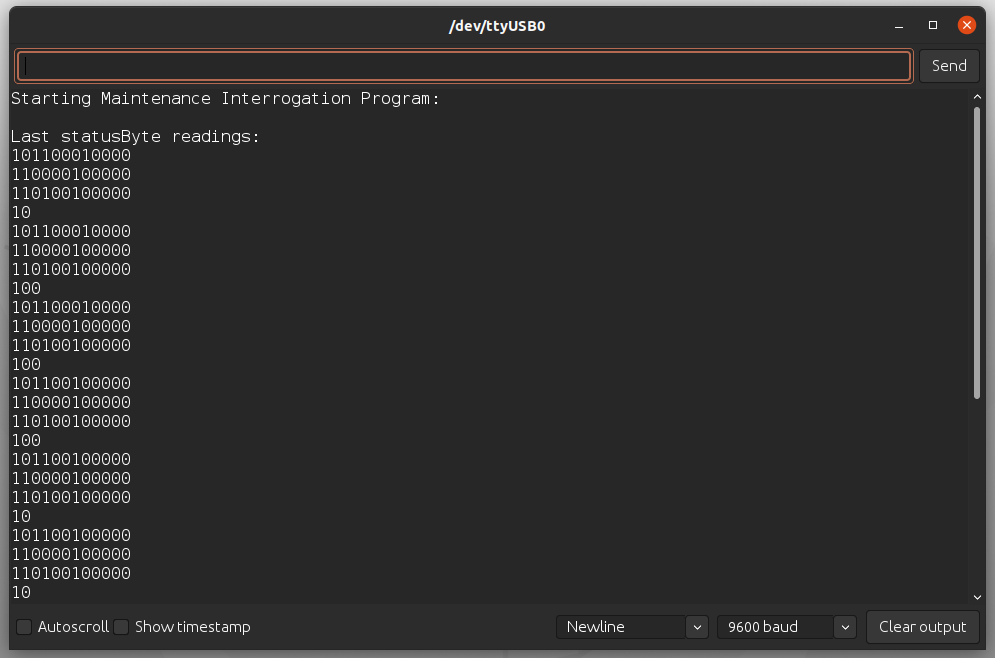
\includegraphics[scale=0.35]{maintenance-interrogation}
\centering
\caption{Maintenance Interrogation program}
\label{fig:maintenance}
\end{figure}

\begin{figure}[h]
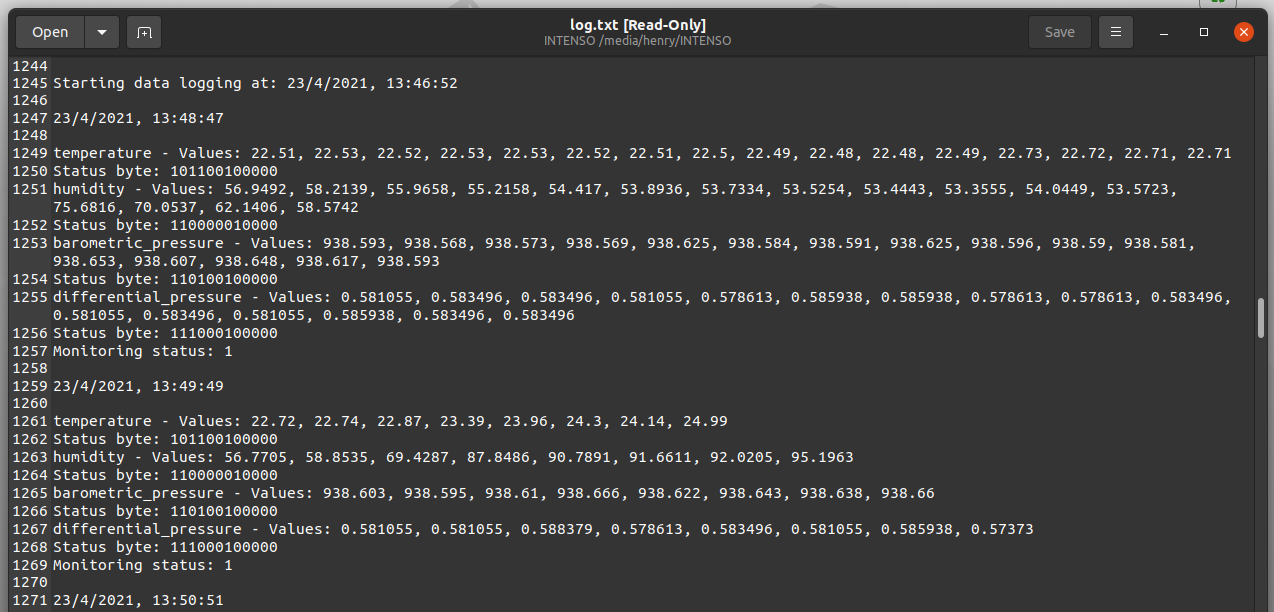
\includegraphics[scale=0.35]{log}
\centering
\caption{Sample readings logged to microSD card}
\label{fig:log}
\end{figure}

\subsubsection{Flash memory}

In Figure \ref{fig:maintenance} you can see the last status byte readings stored in flash memory. As you can see in this example, we have a set of three measurements sending data to InfluxDB (the test metrics Test metric 1, Test metric 2 and Test metric 3). Each of them has associated an ID, which is a binary number between 0 and 255 (1 byte), as explained in the memory optimisation section. As those status byte values only have their least significant 12 bits in the serial monitor output, the 4 most significant bits will represent their ID, in this case 1011, 1100, 1101 (11, 12 and 13). This is expected, as the bidirectional map is initialised with only 11 strings, the ones that appear in the system by default in many tasks. This makes the map start adding measurement name from index 11.\par 

As for the least significant 8 bits, bits 3, 4 and 5 will represent the health of the data; while 0, 1 and 2 will not be used, as these bits are allocated to the monitoring status. You can see bits 3, 4 and 5 to be 010, 100, 100. This means that while Test metric 1 has produced values which fall higher than the higher end of the ``healthy'' range, Test metric 2 and Test metric 3 have both produced values that fall within the range of values expected.\par

At the end of these 3 Status Byte readings, you can see a final reading indicating the monitoring status, with only 3 possible outcomes: 1, 10, 100 (OK\_, WARNING, ALERT). In this case, after the set of 3 measurements, the monitoring status has been established to be WARNING.\par

\subsubsection{External microSD card}

In Figure \ref{fig:log} you can see the file where the data is logged, called log.txt. It is very easy to evaluate the results of logging into an external microSD card, as you can easily see the output of the code, and you only need to compare that to what you wanted to log. In this case the log file is made of 2 parts. The first one contains the start of the logging when the code is first run. After this line of text, the other section of this file will be the periodic logging. In this section we will log all the raw values that were then processed and sent to InfluxDB. This gives us a way of further monitoring the system, as while we log everything that we log to flash memory, the raw data lost when pre-processing now can be stored, which will help for possible further analysis.

\subsection{Reflection and Conclusions}

During my final year at university, I managed to plan, design and successfully implement an IoT project with a monitoring system able to provide very useful information and make appropriate decisions about the environmental parameters of a room / building. The final version manages to develop and implement most of the functionalities listed in the requirements, and is able to take some of the load from the staff members.\par 

Reflecting on how it all went throughout the year, I am aware that there are things I could have done better. The lack of fixed deadlines at some points of the year or the small amount of project planning (which should have been a main focus of the project since the beginning) were important issues that negatively affected the progress on the project. At the beginning of the year, a considerably large amount of time was put into selecting the right choices for the hardware components, and lots of time was wasted as I could not start implementing anything until I received the different parts. Had I organised my ideas better, I would have made more progress at the beginning of the year.\par

Using both InfluxDB and Grafana was also a challenge, specially at the beginning of the project. I had no previous experience working with database management systems, and was very new to the concept of time series databases. As I had very little experience with networks and HTTP requests, I spent some valuable time learning how to use them effectively and how to integrate them into the project. I used Postman in order to gain some understanding about IP addresses and requests over the network, and I read InfluxDB documentation and Grafana documentation in order to be able to understand how they operate and how they are integrated into a system such as this one.\par

Another challenge I encountered was the lack of information regarding memory optimisation that I was able to find. This topic was the hardest for me to implement, as I had to fully understand how the different data points are constructed, how they are stored, and how they are sent to the database. After learning about the whole process, I managed to figure out the key places where data was being wasted and therefore managed to implement a solution that could address that problem. However, I think that section has plenty of room for improvement, as I feel that the section could have been covered in more depth. I am sure it will be a great starting point for future developments.\par  

Originally, this project was meant to be running in a server of the Manchester CMN. Due to Covid-19 restrictions, it was not possible to access the building or accessing the server. This resulted in many challenges regarding the security of the original system not being able to be properly assessed. Looking towards the future, a secure integration of the system into the server should also be a priority for future developments of this project. 

On another note, even though I had no background or experience working in the field of IoT or working with microcontrollers, I was surprised to see that Arduino-compatible microcontrollers offer a very simple and easy way to create IoT systems, and how they easily integrate lots of different examples of I/O devices, therefore being very versatile devices for lots of different purposes. Their shallow learning curve made it a great choice for beginners, so there were no real difficulties when learning how to use them for the first time.\par


\newpage
\printbibliography

\end{document}
